\documentclass[12pt]{article}
\usepackage{ctex}
\usepackage{graphicx}
\usepackage{indentfirst}
\usepackage{amsmath}
\usepackage{amssymb}

\title{第二周作业报告}
\author{佐藤拓未 20300186002}
\date{}

\begin{document}
	\maketitle
	\begin{center}
		\textbf{第一问}
	\end{center}
	设迭代格式为$x_{n+1}=G(x_n)$,并且有以下不等式$$\vert\vert{G(x)-G(y)}\vert\vert\le\alpha\vert\vert{x-y}\vert\vert\quad\alpha\in{[0,1)}$$
	从而有$$\vert\vert{x_{n+2}-x_{n+1}}\vert\vert\le{\alpha}\vert\vert{x_{n+1}-x_{n}}\vert\vert$$
	固定$n$,并不妨设$p>0$,则
	$$\begin{aligned}
			${\vert\vert}{x_{n+p}-x_{n}}{\vert\vert}&\le\vert\vert{x_{n+p}-x_{n+p-1}}{\vert\vert+......+\vert\vert}{x_{n+1}-x_{n}}{\vert\vert}$\\
			$&\le{\alpha^{n+p-1}}\vert\vert{x_1-x_0}\vert\vert+......+{\alpha^n}}\vert\vert{x_1-x_0}\vert\vert$\\
			$&=\frac{\alpha^n(1-\alpha^p)}{1-\alpha}\vert\vert{x_1-x_0}\vert\vert$
		\end{aligned}$$
	从而有$\{x_n\}$是基本列,从而$\exists{x^*}\quad{s.t.}\lim\limits_{p\rightarrow\infty}x_{p}=x^*$,再由$\lim\limits_{p\rightarrow\infty}x_{n+p}=x^*$
	$$\lim\limits_{p\rightarrow\infty}\vert\vert{x_{n+p}-x_{n}}\vert\vert\le\lim\limits_{p\rightarrow\infty}\frac{\alpha^n(1-\alpha^p)}{1-\alpha}\vert\vert{x_1-x_0}\vert\vert$$
	再由$a^p\rightarrow0$
	$$\vert\vert{x^*-x_n}\vert\vert\le\frac{\alpha^n}{1-\alpha}\vert\vert{x_1-x_0}\vert\vert$$
	\\
	
	\begin{center}
		\textbf{第二问}
	\end{center}
	设$G(x)=e^{-x}$与$F(x)=x-e^{-x}$,有不动点迭代格式$x_{n+1}=G(x_n)$与牛顿迭代法格式$x_{n+1}=x_n-\frac{F(x_n)}{F^{'}(x_n)}$,记对应的迭代程序分别为$\{x^G_n\}_{n=1}^\infty$与$\{x^N_n\}_{n=1}^\infty$,并利用MATLAB绘制并对比两迭代法:
	\begin{figure}[h]
		\centering
		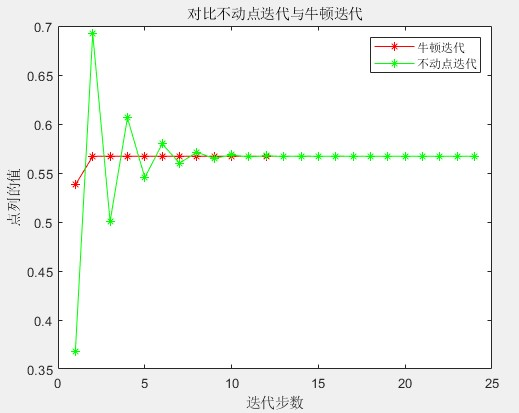
\includegraphics[width=1\textwidth]{图1}
		\caption{红色点列对应了牛顿迭代,绿色点列对应了不动点迭代,初值为1}
	\end{figure}
	\\可以发现牛顿迭代法的收敛速度更快,按照题目要求,给出误差:
	$$
		\begin{aligned}
			$\vert{x^G_{24}}-x^*\vert&\approx4.5769\times10^{-7}$\\
			$\vert{x^N_{4}}-x^*\vert&\approx1.1102\times10^{-16}$\\
			$\vert{x^N_{3}}-x^*\vert&\approx1.5630\times10^{-4}$
		\end{aligned}
	$$
	当初值$x^G_1=x^N_1=1$时,不动点迭代的第24步迭代的精度介于牛顿迭代法的第3与第4步迭代的精度之间。\\
	定性考虑:记$\phi(x)=x-\frac{F(x)}{F^{'}(x)}$,当不动点$x^*$仅是$F(x)$的单根时,考虑在$x^*$的泰勒展开
	$$\phi(x)=\phi(x^*)+{\phi^'}(x^*)(x-x^*)+\frac{1}{2}{\phi^{''}}(\zeta)(x-x^*)^2$$
	而${\phi^'}(x)=\frac{F(x){F^{''}}(x)}{{F^'}(x)^2}$,从而${\phi^'}(x^*)=0$,故有
	$$\phi(x)-\phi(x^*)=\frac{1}{2}{\phi^{''}}(\zeta)(x-x^*)^2$$
	上式意味着当不动点$x^*$为$F(x)$的单根时,牛顿迭代法具有局部二阶收敛,从而相较于不动点迭代,其收敛速度更快。\\
	
	\begin{center}
		\textbf{第三问}
	\end{center}
	设空间维数为$n$,不妨先考虑$\vert\vert{x}\vert\vert_{l_q}=1$
	$$1=\vert\vert{x}\vert\vert_{l_q}^q=\sum_{i=1}^{n}{\vert{x_i}\vert^q}$$
	从而可得$$\vert{x_i}\vert\le1$$
	由于$1\le{p}\le{q}$,可知$\vert{x_i}\vert^q\le\vert{x_i}\vert^p$,故$$\quad\quad1=\vert\vert{x}\vert\vert_{l_q}=(\sum_{i=1}^{n}{\vert{x_i}\vert^q})^\frac{1}{q}\le(\sum_{i=1}^{n}{\vert{x_i}\vert^p})^\frac{1}{q}=(\sum_{i=1}^{n}{\vert{x_i}\vert^p})^{\frac{1}{p}\cdot\frac{p}{q}}\le(\sum_{i=1}^{n}{\vert{x_i}\vert^p})^\frac{1}{p}=\vert\vert{x}\vert\vert_{l_p}$$
	$\forall{y}\in\mathbb{R}^n: \frac{y}{\vert\vert{y}\vert\vert}_{l_q}$的$q-$范数是$1$,代入上式可得$$\vert\vert{y}\vert\vert_{l_q}\le\vert\vert{y}\vert\vert_{l_p}$$
	另一方面,由Hölder不等式$$\sum_{i=1}^n\vert{x_i}\vert^p\le(\sum_{i=1}^n\vert{x_i}\vert^{p\cdot\frac{q}{p}})^\frac{p}{q}\cdot(\sum_{i=1}^n1^\frac{q}{q-p})^\frac{q-p}{q}$$
	从而$$\vert\vert{x}\vert\vert_{l_p}\le\vert\vert{x}\vert\vert_{l_q}\cdot{n^{\frac{1}{p}-\frac{1}{q}}}$$
	综上所述$$\vert\vert{x}\vert\vert_{l_q}\le\vert\vert{x}\vert\vert_{l_p}\le\vert\vert{x}\vert\vert_{l_q}\cdot{n^{\frac{1}{p}-\frac{1}{q}}}$$


\end{document}